\documentclass[11pt]{article}
\usepackage[margin=0.7in]{geometry}
\usepackage{amsmath,amssymb}
\usepackage{enumitem}
\usepackage{tikz}
\usepackage{pgfplots}
\pgfplotsset{compat=1.18}
\usepackage{fancyhdr}
\usepackage{parskip}
\setlist[enumerate]{leftmargin=*, itemsep=6pt}
\pagestyle{fancy}
\fancyhf{}
\fancyfoot[L]{\small\textit{en}Vision\textsuperscript{\textregistered} Algebra 2}
\fancyfoot[C]{\small 1-2 Lesson Quiz, short form}
\fancyfoot[R]{\small\thepage}
\renewcommand{\headrulewidth}{0pt}
\newcommand{\choice}[1]{\tikz[baseline=-0.6ex]\node[draw, circle, inner sep=0.6pt, minimum size=3.3mm, font=\scriptsize\bfseries] {#1};\;}
\newcommand{\checkbox}{$\square$\;}
\pgfplotsset{quizgrid/.style={
  axis lines=middle, grid=both, grid style={gray!45},
  ticklabel style={font=\scriptsize, fill=white, inner sep=1pt},
  xlabel={$x$}, ylabel={$y$}, axis line style={thick}, clip=true}}

\begin{document}

\noindent\textbf{Name}\; \rule{6cm}{0.4pt} \hfill Period \rule{1.2cm}{0.4pt} \quad Date \rule{2.2cm}{0.4pt}

\vspace{4pt}\noindent\rule{\textwidth}{0.6pt}

\vspace{2pt}\noindent{\LARGE\textbf{1-2 \; Lesson Quiz: Transformations of Functions}} \hfill {\small short form}

\vspace{4pt}\noindent\rule{\textwidth}{0.6pt}

\vspace{6pt}
\begin{minipage}[t]{0.56\textwidth}
\textbf{1.} Select \textbf{all} the transformations of $f(x)=x^2$ that combine to result in the graph of function $g$ at the right.

\vspace{4pt}
\begin{itemize}[leftmargin=1.2em, itemsep=5pt]
\item[] \checkbox \textbf{A.} translation of 1 unit left
\item[] \checkbox \textbf{B.} translation of 1 unit right
\item[] \checkbox \textbf{C.} translation of 2 units down
\item[] \checkbox \textbf{D.} horizontal stretch by a factor of 2
\item[] \checkbox \textbf{E.} vertical stretch by a factor of 2
\item[] \checkbox \textbf{F.} reflection across the $x$-axis
\end{itemize}
\end{minipage}\hfill
\begin{minipage}[t]{0.42\textwidth}
\vspace{-6pt}
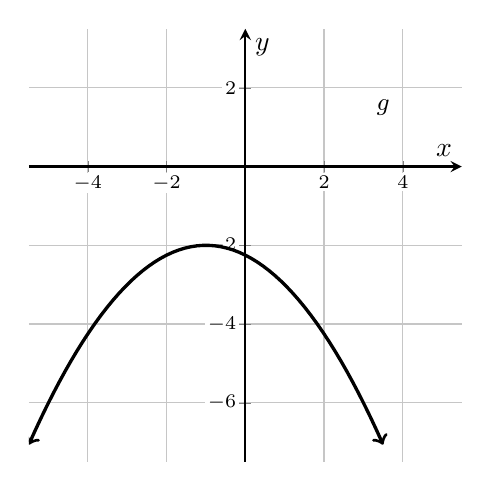
\begin{tikzpicture}
\begin{axis}[quizgrid, xmin=-5.5, xmax=5.5, ymin=-7.5, ymax=3.5,
  xtick={-4,-2,2,4}, ytick={-6,-4,-2,2}, x=0.5cm, y=0.5cm]
\addplot[very thick, domain=-5.5:3.5, samples=60, <->] {-(x+1)^2/4-2};
\node[font=\small] at (axis cs:3.5,1.5) {$g$};
\end{axis}
\end{tikzpicture}
\end{minipage}

\vspace{10pt}\noindent\rule{\textwidth}{0.4pt}

\vspace{6pt}
\begin{minipage}[t]{0.56\textwidth}
\textbf{2.} The graph represents $f$. Graph $g(x)=2f(x-1)$ on the same grid.

\vspace{6pt}
Show your thinking. For one point of $f$, write where it lands on $g$:

\vspace{6pt}
$(\;\rule{1cm}{0.4pt}\;,\;\rule{1cm}{0.4pt}\;)$ on $f$ \;$\longrightarrow$\; $(\;\rule{1cm}{0.4pt}\;,\;\rule{1cm}{0.4pt}\;)$ on $g$

\vspace{8pt}
Which transformation did you do first, the stretch or the shift? Why?

\vspace{4pt}\rule{\linewidth}{0.4pt}

\vspace{10pt}\rule{\linewidth}{0.4pt}
\end{minipage}\hfill
\begin{minipage}[t]{0.42\textwidth}
\vspace{-6pt}
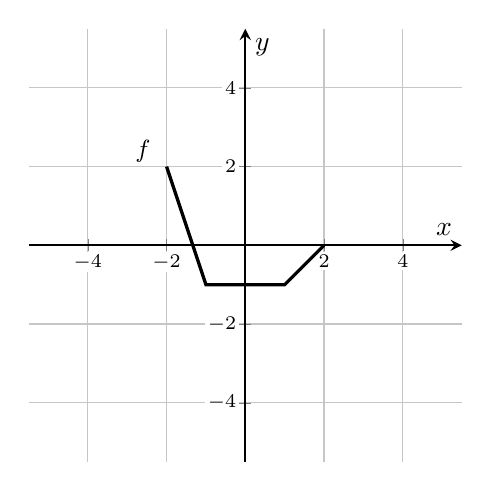
\begin{tikzpicture}
\begin{axis}[quizgrid, xmin=-5.5, xmax=5.5, ymin=-5.5, ymax=5.5,
  xtick={-4,-2,2,4}, ytick={-4,-2,2,4}, minor tick num=1, x=0.5cm, y=0.5cm]
\addplot[very thick] coordinates {(-2,2) (-1,-1) (1,-1) (2,0)};
\node[font=\small] at (axis cs:-2.6,2.4) {$f$};
\end{axis}
\end{tikzpicture}
\end{minipage}

\vspace{10pt}\noindent\rule{\textwidth}{0.4pt}

\vspace{6pt}
\begin{minipage}[t]{0.56\textwidth}
\textbf{3.} The graph of the function $f$ is shown. The domain of $f$ is $[0,50]$. What is the range of $g(x)=4f(x)$?

\vspace{4pt}
\begin{itemize}[leftmargin=1.2em, itemsep=5pt]
\item[] \choice{A} $[0,50]$
\item[] \choice{B} $[0,70]$
\item[] \choice{C} $[0,1.75]$
\item[] \choice{D} $[0,7]$
\end{itemize}

\vspace{4pt}
Explain in one sentence why the domain of $g$ is still $[0,50]$:

\vspace{4pt}\rule{\linewidth}{0.4pt}
\end{minipage}\hfill
\begin{minipage}[t]{0.42\textwidth}
\vspace{-6pt}
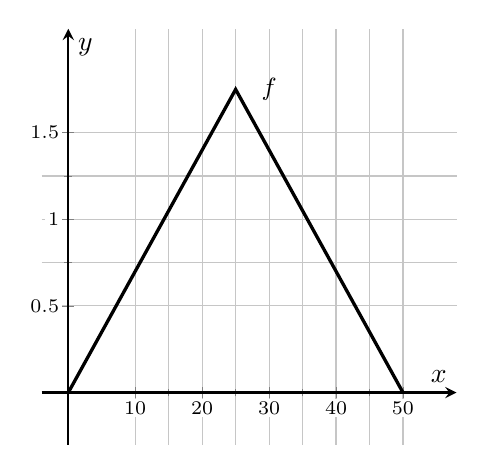
\begin{tikzpicture}
\begin{axis}[quizgrid, xmin=-4, xmax=58, ymin=-0.3, ymax=2.1,
  xtick={10,20,30,40,50}, ytick={0.5,1,1.5}, minor x tick num=1, minor y tick num=1,
  x=0.085cm, y=2.2cm, xlabel={$x$}, ylabel={$y$}]
\addplot[very thick] coordinates {(0,0) (25,1.75) (50,0)};
\node[font=\small] at (axis cs:30,1.75) {$f$};
\end{axis}
\end{tikzpicture}
\end{minipage}

\vfill
\noindent\textbf{Scoring:} Question 2 and Question 3 are 10 points each. Question 1 is a bonus of up to 5 points (all four correct boxes, none wrong). Total out of 20.

\newpage
\noindent{\LARGE\textbf{1-2 Lesson Quiz, short form: answer key}}

\vspace{4pt}\noindent\rule{\textwidth}{0.6pt}

\begin{enumerate}
\item \textbf{A, C, D, F.} Vertex $(-1,-2)$: left 1, down 2. Opens down: reflection across the $x$-axis. Wider than $x^2$ (passes through $(1,-3)$, so $a=-\tfrac14$): horizontal stretch by 2. Savvas quiz item 1, DOK 2, standard HSF.BF.B.3. \textbf{Bonus 5:} all four boxes and no extra box; 3 for three correct and none wrong; 0 otherwise.
\item \textbf{$g$ joins $(-1,4)$, $(0,-2)$, $(2,-2)$, $(3,0)$.} Each point $(x,y)$ of $f$ goes to $(x+1,\,2y)$. Either order of stretch and shift gives the same graph here because the stretch is vertical and the shift is horizontal; accept either order with a reason. Savvas quiz item 3, DOK 1, HSF.BF.B.3. \textbf{10 points:} 6 for the four correct points, 2 for the mapped point, 2 for the order explanation.
\item \textbf{D, $[0,7]$.} The maximum of $f$ is $1.75$ and $4(1.75)=7$. The domain is unchanged because $4f(x)$ multiplies outputs, not inputs. Savvas quiz item 5, DOK 2, HSF.IF.B.5 with HSF.BF.B.3. \textbf{10 points:} 7 for D, 3 for the domain sentence naming outputs versus inputs.
\end{enumerate}

\textbf{Items left off this form} (available for a retake or Form B): Savvas item 2, equation of $2x^2+3x-1$ reflected across the $y$-axis (answer C, $2x^2-3x-1$); Savvas item 4, the leaking-bucket translation (answer D, $|x-3|$).

\textbf{IXL replacement:} SmartScore 70 or above on NNY, RSN and KQL replaces this quiz with 20/20.

\end{document}
